% Copyright 2006 by Till Tantau
%
% This file may be distributed and/or modified
%
% 1. under the LaTeX Project Public License and/or
% 2. under the GNU Free Documentation License.
%
% See the file doc/generic/pgf/licenses/LICENSE for more details.


\section{Arrow Tips}
\label{section-arrows}


\subsection{Overview}

\subsubsection{When Does PGF Draw Arrow Tips?}

\pgfname\ offers an interface for placing \emph{arrow tips} at the end
of lines. The interface works as follows:

\begin{enumerate}
\item
  You (or someone else) assigns a name to a certain kind of arrow
  tips. For example, the
  arrow tip |latex| is the arrow tip used by the standard \LaTeX\
  picture environment; the arrow tip |to| looks like the tip of the
  arrow in \TeX's |\to| command; and so on.

  This is done once at the beginning of the document.
\item
  Inside some picture, at some point you specify that in the current
  scope from now on you would like tips of, say, kind |to| to be added
  at the end and/or beginning of all paths.

  When an arrow kind has been installed and when \pgfname\ is about to
  stroke a path, the following things happen:
  \begin{enumerate}
  \item
    The beginning and/or end of the path is shortened appropriately.
  \item
    The path is stroked.
  \item
    The arrow tip is drawn at the beginning and/or end of the path,
    appropriately rotated and appropriately resized.
  \end{enumerate}
\end{enumerate}

In the above description, there are a number of ``appropriately.''
The exact details are not quite trivial and described later on.


\subsubsection{Meta-Arrow Tips}

In \pgfname, arrows are ``meta-arrows'' in the same way that fonts in
\TeX\ are ``meta-fonts.'' When a meta-arrow is resized, it is not
simply scaled, but a possibly complicated transformation is applied to
the size.

A meta-font is not one particular font at a specific size with a
specific stroke width (and with a large number of other parameters
being fixed). Rather, it is a ``blueprint'' (actually, more like a
program) for generating such a font at a particular size and
width. This allows the designer of a meta-font to make sure that, say,
the font is somewhat thicker and wider at very small sizes. To
appreciate the difference: Compare the following texts: ``Berlin'' and
``\tikz{\node [scale=2,inner sep=0pt,outer sep=0pt]{\tiny
    Berlin};}''. The first is a ``normal'' text, the second is the tiny
version scaled by a factor of two. Obviously, the first look
better. Now, compare  ``\tikz{\node [scale=.5,inner sep=0pt,outer
  sep=0pt]{Berlin};}'' and ``{\tiny Berlin}''. This time, the normal
text was scaled down, while the second text is a ``normal'' tiny
text. The second text is easier to read.

\pgfname's meta-arrows work in a similar fashion: The shape of an
arrow tip can vary according to the line width of the arrow tip is
used. Thus, an arrow tip drawn at a line width of 5pt will typically
\emph{not} be five times as large as an arrow tip of line width
1pt. Instead, the size of the arrow will get bigger only slowly as the
line width increases.

To appreciate the difference, here are the |latex| and |to| arrows, as
drawn by \pgfname\ at four different sizes:

\medskip
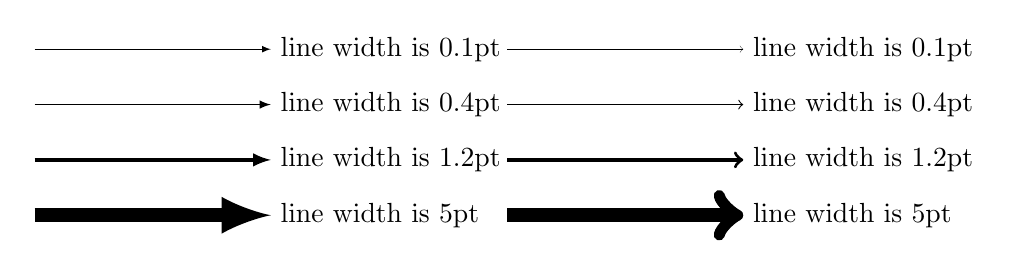
\begin{tikzpicture}
  \draw[-latex,line width=0.1pt] (0pt,0ex) -- +(3,0)  node[thin,right] {line width is 0.1pt};
  \draw[-latex,line width=0.4pt] (0pt,-2em) -- +(3,0) node[thin,right] {line width is 0.4pt};
  \draw[-latex,line width=1.2pt] (0pt,-4em) -- +(3,0) node[thin,right] {line width is 1.2pt};
  \draw[-latex,line width=5pt]   (0pt,-6em) -- +(3,0) node[thin,right] {line width is 5pt};

  \draw[-to,line width=0.1pt] (6cm,0ex) -- +(3,0)  node[thin,right] {line width is 0.1pt};
  \draw[-to,line width=0.4pt] (6cm,-2em) -- +(3,0) node[thin,right] {line width is 0.4pt};
  \draw[-to,line width=1.2pt] (6cm,-4em) -- +(3,0) node[thin,right] {line width is 1.2pt};
  \draw[-to,line width=5pt]   (6cm,-6em) -- +(3,0) node[thin,right] {line width is 5pt};
\end{tikzpicture}

\medskip
Here, by comparison, is the same arrow when it is simply ``resized''
(as done by some programs):

\pgfarrowsdeclare{bad latex}{bad latex}
{
  \pgfarrowsleftextend{-1\pgflinewidth}
  \pgfarrowsrightextend{9\pgflinewidth}
}
{
  \pgfpathmoveto{\pgfpoint{9\pgflinewidth}{0pt}}
  \pgfpathcurveto
  {\pgfpoint{6.3333\pgflinewidth}{.5\pgflinewidth}}
  {\pgfpoint{2\pgflinewidth}{2\pgflinewidth}}
  {\pgfpoint{-1\pgflinewidth}{3.75\pgflinewidth}}
  \pgfpathlineto{\pgfpoint{-1\pgflinewidth}{-3.75\pgflinewidth}}
  \pgfpathcurveto
  {\pgfpoint{2\pgflinewidth}{-2\pgflinewidth}}
  {\pgfpoint{6.3333\pgflinewidth}{-.5\pgflinewidth}}
  {\pgfpoint{9\pgflinewidth}{0pt}}
  \pgfusepathqfill
}

\pgfarrowsdeclare{bad to}{bad to}
{
  \pgfarrowsleftextend{-2\pgflinewidth}
  \pgfarrowsrightextend{\pgflinewidth}
}
{
  \pgfsetlinewidth{0.8\pgflinewidth}
  \pgfsetdash{}{0pt}
  \pgfsetroundcap
  \pgfsetroundjoin
  \pgfpathmoveto{\pgfpoint{-3\pgflinewidth}{4\pgflinewidth}}
  \pgfpathcurveto
  {\pgfpoint{-2.75\pgflinewidth}{2.5\pgflinewidth}}
  {\pgfpoint{0pt}{0.25\pgflinewidth}}
  {\pgfpoint{0.75\pgflinewidth}{0pt}}
  \pgfpathcurveto
  {\pgfpoint{0pt}{-0.25\pgflinewidth}}
  {\pgfpoint{-2.75\pgflinewidth}{-2.5\pgflinewidth}}
  {\pgfpoint{-3\pgflinewidth}{-4\pgflinewidth}}
  \pgfusepathqstroke
}

\medskip
\begin{tikzpicture}
  \draw[-bad latex,line width=0.1pt] (0pt,0ex) -- +(3,0)  node[thin,right] {line width is 0.1pt};
  \draw[-bad latex,line width=0.4pt] (0pt,-2em) -- +(3,0) node[thin,right] {line width is 0.4pt};
  \draw[-bad latex,line width=1.2pt] (0pt,-4em) -- +(3,0) node[thin,right] {line width is 1.2pt};
  \draw[-bad latex,line width=5pt]   (0pt,-6em) -- +(3,0) node[thin,right] {line width is 5pt};

  \draw[-bad to,line width=0.1pt] (6cm,0ex) -- +(3,0)  node[thin,right] {line width is 0.1pt};
  \draw[-bad to,line width=0.4pt] (6cm,-2em) -- +(3,0) node[thin,right] {line width is 0.4pt};
  \draw[-bad to,line width=1.2pt] (6cm,-4em) -- +(3,0) node[thin,right] {line width is 1.2pt};
  \draw[-bad to,line width=5pt]   (6cm,-6em) -- +(3,0) node[thin,right] {line width is 5pt};
\end{tikzpicture}

\bigskip
As can be seen, simple scaling produces arrow tips that are way too
large at larger sizes and way too small at smaller sizes.

In addition to the line width, other options may also influence the
appearance of an arrow tip. In particular, the width of the inner line
(the line used to create the effect of a double line) influences arrow
tips as well as other options that are specific to the arrow tip.



\subsection{Declaring an Arrow Tip Kind}

To declare an arrow kind ``from scratch,'' the following command is
used:

\begin{command}{\pgfarrowsdeclare\marg{start name}\marg{end
      name}\marg{extend code}\marg{arrow tip code}}
  This command declares a new arrow kind. An arrow kind has two names,
  which will typically be the same. When the arrow tip needs to be
  drawn, the \meta{arrow tip code} will be invoked, but the canvas
  transformation is setup beforehand to a rotation such that when an
  arrow tip pointing right is specified, the arrow tip that is
  actually drawn points in the direction of the line.

  \medskip
  \textbf{Naming the arrow kind.}
  The \meta{start name} is the name
  used for the arrow tip when it is at the start of a path, the \meta{end
    name} is the name used at the end of a path. For example, the
  arrow kind that looks like a parenthesis has the \meta{start
    name} |(| and the \meta{end name} |)| so that you can say
  |\pgfsetarrows{(-)}| to specify that you want parenthesis arrows and
  both ends.

  The \meta{end name} and \meta{start name} can be quite arbitrary and
  may contain spaces.

  \medskip
  \textbf{Basics of the arrow tip code.}
  Let us next have a look at the \meta{arrow tip code}. This code will
  be used to draw the arrow tip when \pgfname\ thinks this is
  necessary. The code should draw an arrow that ``points right,''
  which means that is should draw an arrow at the end of a line coming
  from the left and ending at the origin.

  As an example, suppose we wanted to declare an arrow tip consisting
  of two arcs, that is, we want the arrow tip to look more or less
  like the red part of the following picture:
\begin{codeexample}[]
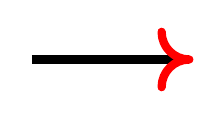
\begin{tikzpicture}[line width=3pt]
  \draw (-2,0) -- (0,0);
  \draw[red,line join=round,line cap=round]
        (-10pt,10pt) arc (180:270:10pt) arc (90:180:10pt);
\end{tikzpicture}
\end{codeexample}

  We could use the following as \meta{arrow tip code} for this:
\begin{codeexample}[code only]
\pgfarrowsdeclare{arcs}{arcs}{...}
{
  \pgfsetdash{}{0pt} % do not dash
  \pgfsetroundjoin   % fix join
  \pgfsetroundcap    % fix cap
  \pgfpathmoveto{\pgfpoint{-10pt}{10pt}}
  \pgfpatharc{180}{270}{10pt}
  \pgfpatharc{90}{180}{10pt}
  \pgfusepathqstroke
}
\end{codeexample}

  Indeed, when the |...| is set appropriately (in a moment), we can
  write the following:
\pgfarrowsdeclare{arcs}{arcs}{\pgfarrowsleftextend{0pt}\pgfarrowsrightextend{0pt}}
{
  \pgfsetdash{}{0pt} % do not dash
  \pgfsetroundjoin   % fix join
  \pgfsetroundcap    % fix cap
  \pgfpathmoveto{\pgfpoint{-10pt}{10pt}}
  \pgfpatharc{180}{270}{10pt}
  \pgfpatharc{90}{180}{10pt}
  \pgfusepathqstroke
}
\begin{codeexample}[]
\begin{tikzpicture}
  \draw[-arcs,line width=3pt] (-2,0)  -- (0,0);
  \draw[arcs-arcs,line width=1pt] (-2,-1.5) -- (0,-1);
  \useasboundingbox (-2,-2) rectangle (0,0.75);
\end{tikzpicture}
\end{codeexample}

  As can be seen in the second example, the arrow tip is automatically
  rotated as needed when the arrow is drawn. This is achieved by a
  canvas rotation.

  \medskip
  \textbf{Special considerations about the arrow tip code.}
  There are several things you need to be aware of when designing
  arrow tip code:
  \begin{itemize}
  \item
    Inside the code, you may not use the |\pgfusepath|
    command. The reason is that this command internally calls arrow
    construction commands, which is something you obviously do not want
    to happen.

    Instead of |\pgfusepath|, use the quick versions. Typically, you
    will use |\pgfusepathqstroke|, |\pgfusepathqfill|, or
    |\pgfusepathqfillstroke|.
  \item
    The code will be executed only once, namely the first time the
    arrow tip needs to be drawn. The resulting low-level driver
    commands are protocolled and stored away. In all subsequent
    uses of the arrow tip, the protocolled code is directly inserted.
  \item
    However, the code will be executed anew for each line width. Thus,
    an arrow of line width 2pt may result in a different protocol than
    the same arrow for a line width of 0.4pt.
  \item
    If you stroke the path that you construct, you should first set
    the dashing to solid and setup fixed joins and caps, as
    needed. This will ensure that the arrow tip will always look the
    same.
  \item
    When the arrow tip code is executed, it is automatically put
    inside a low-level scope, so nothing will ``leak out'' from the
    scope.
  \item
    The high-level coordinate transformation matrix will be set to the
    identity matrix when the code is executed for the first time.
  \end{itemize}

  \medskip
  \textbf{Designing meta-arrows.}
  The \meta{arrow tip code} should adjust the size of the arrow in
  accordance with the line width. For a small line width, the arrow
  tip should be small, for a large line width, it should be
  larger. However, the size of the arrow typically \emph{should not}
  grow in direct proportion to the line width. On the other hand, the
  size of the arrow head typically \emph{should} grow ``a bit'' with
  the line width.

  For these reasons, \pgfname\ will not simply executed your arrow
  code within a scaled scope, where the scaling depends on the line
  width. Instead, your \meta{arrow tip code} is reexecuted again for
  each different line width.

  In our example, we could use the following code for the new arrow
  tip kind |arc'| (note the prime):
\begin{codeexample}[code only]
\newdimen\arrowsize
\pgfarrowsdeclare{arcs'}{arcs'}{...}
{
  \arrowsize=0.2pt
  \advance\arrowsize by .5\pgflinewidth
  \pgfsetdash{}{0pt} % do not dash
  \pgfsetroundjoin   % fix join
  \pgfsetroundcap    % fix cap
  \pgfpathmoveto{\pgfpoint{-4\arrowsize}{4\arrowsize}}
  \pgfpatharc{180}{270}{4\arrowsize}
  \pgfpatharc{90}{180}{4\arrowsize}
  \pgfusepathqstroke
}
\end{codeexample}
\newdimen\arrowsize
\pgfarrowsdeclare{arcs'}{arcs'}{\pgfarrowsleftextend{0pt}\pgfarrowsrightextend{0pt}}
{
  \arrowsize=0.2pt
  \advance\arrowsize by .5\pgflinewidth
  \pgfsetdash{}{0pt} % do not dash
  \pgfsetroundjoin   % fix join
  \pgfsetroundcap    % fix cap
  \pgfpathmoveto{\pgfpoint{-4\arrowsize}{4\arrowsize}}
  \pgfpatharc{180}{270}{4\arrowsize}
  \pgfusepathqstroke
  \pgfpathmoveto{\pgfpointorigin}
  \pgfpatharc{90}{180}{4\arrowsize}
  \pgfusepathqstroke
}
\begin{codeexample}[]
\begin{tikzpicture}
  \draw[-arcs',line width=3pt] (-2,0)  -- (0,0);
  \draw[arcs'-arcs',line width=1pt] (-2,-1.5) -- (0,-1);
  \useasboundingbox (-2,-1.75) rectangle (0,0.5);
\end{tikzpicture}
\end{codeexample}

  However, sometimes, it can also be useful to have arrows that do not
  resize at all when the line width changes. This can be achieved by
  giving absolute size coordinates in the code, as done for |arc|. On
  the other hand, you can also have the arrow resize linearly with the
  line width by specifying all coordinates as multiples of
  |\pgflinewidth|.

  \medskip
  \textbf{The left and right extend.}
  Let us have another look at the exact left and right ``ends'' of our
  arrow tip. Let us draw the arrow tip |arc'| at a very large size:

\begin{codeexample}[]
\begin{tikzpicture}
  \draw[help lines] (-2,-1) grid (1,1);
  \draw[line width=10pt,-arcs'] (-2,0) -- (0,0);
  \draw[line width=2pt,white] (-2,0) -- (0,0);
\end{tikzpicture}
\end{codeexample}

  As one can see, the arrow tip does not ``touch'' the origin as it
  should, but protrudes a little over the origin. One remedy to this
  undesirable effect is to change the code of the arrow tip such that
  everything is shifted half an |\arrowsize| to the left. While this
  will cause the arrow tip to touch the origin, the line itself will
  then interfere with the arrow: The arrow tip will be partly
  ``hidden'' by the line itself.

  \pgfname\ uses a different approach to solving the problem: The
  \meta{extend code} argument can be used to ``tell'' \pgfname\ how
  much the arrow protrudes over the origin. The argument is also used
  to tell \pgfname\ where the ``left'' end of the arrow is. However,
  this number is important only when the arrow is being reversed or
  composed with other arrow tips.

  Once \pgfname\ knows the right extend of an arrow kind, it can
  \emph{shorten} lines by this amount when drawing arrows.

  Here is a picture that shows what the visualizes the extends. The
  arrow tip itself is shown in red once more:

  \medskip
  \begin{tikzpicture}
    \draw[line width=1cm,-arcs',red] (-6,0) -- (0,0);
    \draw[line width=1cm,black]      (-6,0) -- (0,0);
    \draw[help lines] (-6,0) -- (2,0)     (0,-3) -- (0,3) coordinate (a);
    \draw[help lines,xshift=0.5cm]        (0,-3) -- (0,3) coordinate (b);
    \draw[help lines,xshift=-2.5cm-0.8pt] (0,-3) -- (0,3) coordinate (c);

    \coordinate (xline 1) at (0,1.5);
    \coordinate (xline 2) at (0,2.8);

    \draw[|->|] (xline 1 -| a) -- node[above=2pt] {right extend} (xline 1 -| b);
    \draw[|<-|] (xline 2 -| c) -- node[above=2pt] {left extend}  (xline 2 -| a);

    \draw (0,0) -- (1,-1) node[below right] {origin};
   \end{tikzpicture}


  The \meta{extend code} is normal \TeX\ code that is executed
  whenever \pgfname\ wants to know how far the arrow tip will protrude
  to the right and left. The code should call the following two
  commands: \declare{|\pgfarrowsrightextend|} and
  \declare{|\pgfarrowsleftextend|}. Both arguments take one argument
  that specifies the size. Here is the final code for the |arc''| arrow
  tip:
\begin{codeexample}[]
\pgfarrowsdeclare{arcs''}{arcs''}
{
  \arrowsize=0.2pt
  \advance\arrowsize by .5\pgflinewidth
  \pgfarrowsleftextend{-4\arrowsize-.5\pgflinewidth}
  \pgfarrowsrightextend{.5\pgflinewidth}
}
{
  \arrowsize=0.2pt
  \advance\arrowsize by .5\pgflinewidth
  \pgfsetdash{}{0pt} % do not dash
  \pgfsetroundjoin   % fix join
  \pgfsetroundcap    % fix cap
  \pgfpathmoveto{\pgfpoint{-4\arrowsize}{4\arrowsize}}
  \pgfpatharc{180}{270}{4\arrowsize}
  \pgfusepathqstroke
  \pgfpathmoveto{\pgfpointorigin}
  \pgfpatharc{90}{180}{4\arrowsize}
  \pgfusepathqstroke
}
\begin{tikzpicture}
  \draw[help lines] (-2,-1) grid (1,1);
  \draw[line width=10pt,-arcs''] (-2,0) -- (0,0);
  \draw[line width=2pt,white] (-2,0) -- (0,0);
\end{tikzpicture}
\end{codeexample}

  \medskip
  \textbf{Taking inner lines into account.}
  In addition to the line width, there is another parameter that (may)
  influence the way an arrow looks: The inner line width, which is the
  line width of the second line that is stroked on top of a normal
  line in order to create the effect of a ``double'' line. When this
  line width changes, the arrow tip code is also reexecuted (and
  cached), so your code may depend on the current value of the inner
  line width.

  The following example shows how this works. The |implies| arrow
  defined below has to setup the line width not for the ``main'' line
  width, but for the main line width minus the inner line width,
  divided by~2.
\begin{codeexample}[code only]
\pgfarrowsdeclare{implies}{implies}{...}
{
  \pgfmathsetlength{\pgfutil@tempdimb}{.5\pgflinewidth-.5*\pgfinnerlinewidth}%
  \pgfsetlinewidth{\pgfutil@tempdimb}
  \pgfsetdash{}{0pt}
  \pgfsetroundcap
  \pgfsetroundjoin
  \pgfmathsetlength{\pgfutil@tempdima}{.25\pgflinewidth+.25*\pgfinnerlinewidth}%
  \pgfpathmoveto {\pgfpoint{-1.4\pgfutil@tempdima}{2.65\pgfutil@tempdima}}
  \pgfpathcurveto{\pgfpoint{-0.75\pgfutil@tempdima}{1.25\pgfutil@tempdima}}
                 {\pgfpoint{1\pgfutil@tempdima}{0.05\pgfutil@tempdima}}
                 {\pgfpoint{2\pgfutil@tempdima}{0pt}}
  \pgfpathcurveto{\pgfpoint{1\pgfutil@tempdima}{-0.05\pgfutil@tempdima}}
                 {\pgfpoint{-.75\pgfutil@tempdima}{-1.25\pgfutil@tempdima}}
                 {\pgfpoint{-1.4\pgfutil@tempdima}{-2.65\pgfutil@tempdima}}
  \pgfusepathqstroke
}
\end{codeexample}
  Here is the effect for different combinations of line width and
  inner line width:
\begin{codeexample}[]
\begin{tikzpicture}
  \foreach \linewidth in {2,2.4,...,4.4}
    \foreach \innerlinewidth in {0.4,0.8,...,1.8}
    {
      \pgfsetlinewidth{\linewidth pt}
      \pgfsetinnerlinewidth{\innerlinewidth pt}
      \draw [-implies] (\innerlinewidth*50pt,\linewidth*40pt) -- ++(4mm,0);
    }
\end{tikzpicture}
\end{codeexample}

  \medskip
  \textbf{Arrow options.}
  You may wish to have further option influence the appearance of an
  arrow tip. For instance, for a ``pointed'' arrow you may wish to set
  the opening angle of the tip. Then, whenever this option changes
  that arrow tip code also needs to be reexecuted, even though the
  line width has stayed the same.

  You can use the commands |\pgfsetarrowoptions| and
  |\pgfgetarrowoptions| to set such options for an arrow tip. Whenever
  an arrow tip needs to be rendered, it is checked whether the arrow
  tip code has already been executed for the current (expanded) value of the
  options. If so, the cached code is used; otherwise the code is
  executed once more. Naturally, inside the code the current value of
  the arrow options should be taken into account.

  Arrow options can and must be specified individually for each arrow
  type.

  In the following example, we make the arc angle an option.
\begin{codeexample}[]
\pgfarrowsdeclare{var arc}{var arc} % options is an angle
{
  \arrowsize=0.2pt
  \advance\arrowsize by .5\pgflinewidth
  \pgfarrowsleftextend{-4\arrowsize-.5\pgflinewidth}
  \pgfarrowsrightextend{.5\pgflinewidth}
}
{
  \arrowsize=0.2pt
  \advance\arrowsize by .5\pgflinewidth
  \pgfsetdash{}{0pt} % do not dash
  \pgfsetroundjoin   % fix join
  \pgfsetroundcap    % fix cap
  \pgfpathmoveto{\pgfpointorigin}
  \pgfpatharc{-90}{-180+\pgfgetarrowoptions{var arc}}{4\arrowsize}
  \pgfusepathqstroke
  \pgfpathmoveto{\pgfpointorigin}
  \pgfpatharc{90}{180-\pgfgetarrowoptions{var arc}}{4\arrowsize}
  \pgfusepathqstroke
}
\begin{tikzpicture}
  \draw[help lines] (-2,-4) grid (1,4);
  \foreach \option in {-60,-50,...,60}
  {
    \pgfsetarrowoptions{var arc}{\option}
    \draw[ultra thick,-var arc] (-2,\option/15) -- (0,\option/15);
  }
\end{tikzpicture}
\end{codeexample}
\end{command}

\pgfarrowsdeclare{arcs''}{arcs''}
{
  \arrowsize=0.2pt
  \advance\arrowsize by .5\pgflinewidth
  \pgfarrowsleftextend{-4\arrowsize-.5\pgflinewidth}
  \pgfarrowsrightextend{.5\pgflinewidth}
}
{
  \arrowsize=0.2pt
  \advance\arrowsize by .5\pgflinewidth
  \pgfsetdash{}{0pt} % do not dash
  \pgfsetroundjoin   % fix join
  \pgfsetroundcap    % fix cap
  \pgfpathmoveto{\pgfpoint{-4\arrowsize}{4\arrowsize}}
  \pgfpatharc{180}{270}{4\arrowsize}
  \pgfusepathqstroke
  \pgfpathmoveto{\pgfpointorigin}
  \pgfpatharc{90}{180}{4\arrowsize}
  \pgfusepathqstroke
}

\begin{command}{\pgfsetarrowoptions\marg{arrow tip}\marg{text}}
  Sets the options for the \meta{arrow tip} to \meta{text}. The
  default, before any call to this macro is made, is 0.
\end{command}

\begin{command}{\pgfgetarrowoptions\marg{arrow tip}}
  This will expand to the current value of the options for the
  \meta{arrow tip}.
\end{command}



\subsection{Declaring a Derived Arrow Tip Kind}

It is possible to declare arrow kinds in terms of existing ones. For
these command to work correctly, the left and right extends must be
set correctly.

\begin{command}{\pgfarrowsdeclarealias\marg{start name}\marg{end
      name}\marg{old start name}\marg{old end name}}
  This command can be used to create an alias (another name) for an
  existing arrow kind.

\begin{codeexample}[]
\pgfarrowsdeclarealias{<}{>}{arcs''}{arcs''}%
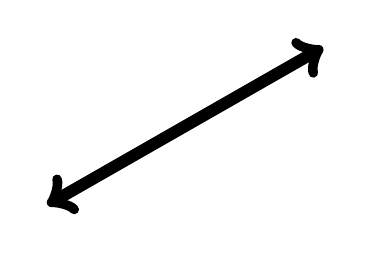
\begin{tikzpicture}
  \pgfsetarrows{<->}
  \pgfsetlinewidth{1ex}
  \pgfpathmoveto{\pgfpointorigin}
  \pgfpathlineto{\pgfpoint{3.5cm}{2cm}}
  \pgfusepath{stroke}
  \useasboundingbox (-0.25,-0.25) rectangle (3.75,2.25);
\end{tikzpicture}
\end{codeexample}
\end{command}


\begin{command}{\pgfarrowsdeclarereversed\marg{start name}\marg{end
      name}\marg{old start name}\marg{old end name}}
  This command creates a new arrow kind that is the ``reverse'' of an
  existing arrow kind. The (automatically cerated) code of the new
  arrow kind will contain a flip of the canvas and the meanings of the
  left and right extend will be reversed.

\begin{codeexample}[]
\pgfarrowsdeclarereversed{arcs reversed}{arcs reversed}{arcs''}{arcs''}%
\begin{tikzpicture}
  \pgfsetarrows{arcs reversed-arcs reversed}
  \pgfsetlinewidth{1ex}
  \pgfpathmoveto{\pgfpointorigin}
  \pgfpathlineto{\pgfpoint{3.5cm}{2cm}}
  \pgfusepath{stroke}
  \useasboundingbox (-0.25,-0.25) rectangle (3.75,2.25);
\end{tikzpicture}
\end{codeexample}
\end{command}



\begin{command}{\pgfarrowsdeclarecombine\opt{|*|}\opt{\oarg{offset}}\marg{start
      name}\marg{end name}\marg{first start name}\marg{first end
      name}\penalty0\marg{second start name}\marg{second end name}}
  This command creates a new arrow kind that combines two existing
  arrow kinds. The first arrow kind is the ``innermost'' arrow kind,
  the second arrow kind is the ``outermost.''

  The code for the combined arrow kind will install a canvas
  translation before the innermost arrow kind in drawn. This
  translation is calculated such that the right tip of the innermost
  arrow touches the right  end of the outermost arrow. The optional
  \meta{offset} can be used to increase (or decrease) the distance
  between the inner and outermost arrow.

\begin{codeexample}[]
\pgfarrowsdeclarecombine[\pgflinewidth]
  {combined}{combined}{arcs''}{arcs''}{latex}{latex}%
\begin{tikzpicture}
  \pgfsetarrows{combined-combined}
  \pgfsetlinewidth{1ex}
  \pgfpathmoveto{\pgfpointorigin}
  \pgfpathlineto{\pgfpoint{3.5cm}{2cm}}
  \pgfusepath{stroke}
  \useasboundingbox (-0.25,-0.25) rectangle (3.75,2.25);
\end{tikzpicture}
\end{codeexample}

  In the star variant, the end of the line is not in the outermost
  arrow, but inside the innermost arrow.

\begin{codeexample}[]
\pgfarrowsdeclarecombine*[\pgflinewidth]
  {combined'}{combined'}{arcs''}{arcs''}{latex}{latex}%
\begin{tikzpicture}
  \pgfsetarrows{combined'-combined'}
  \pgfsetlinewidth{1ex}
  \pgfpathmoveto{\pgfpointorigin}
  \pgfpathlineto{\pgfpoint{3.5cm}{2cm}}
  \pgfusepath{stroke}
  \useasboundingbox (-0.25,-0.25) rectangle (3.75,2.25);
\end{tikzpicture}
\end{codeexample}
\end{command}


\begin{command}{\pgfarrowsdeclaredouble\opt{\oarg{offset}}\marg{start
      name}\marg{end name}\marg{old start name}\marg{old end
      name}}
  This command is a shortcut for combining an arrow kind with itself.

\begin{codeexample}[]
\pgfarrowsdeclaredouble{<<}{>>}{arcs''}{arcs''}%
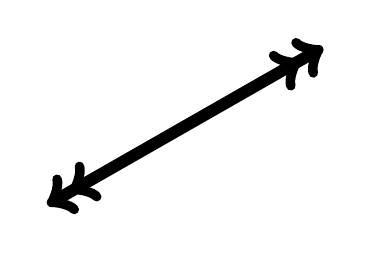
\begin{tikzpicture}
  \pgfsetarrows{<<->>}
  \pgfsetlinewidth{1ex}
  \pgfpathmoveto{\pgfpointorigin}
  \pgfpathlineto{\pgfpoint{3.5cm}{2cm}}
  \pgfusepath{stroke}
  \useasboundingbox (-0.25,-0.25) rectangle (3.75,2.25);
\end{tikzpicture}
\end{codeexample}
\end{command}


\begin{command}{\pgfarrowsdeclaretriple\opt{\oarg{offset}}\marg{start
      name}\marg{end name}\marg{old start name}\marg{old end
      name}}
  This command is a shortcut for combining an arrow kind with itself
  and then again.

\begin{codeexample}[]
\pgfarrowsdeclaretriple{<<<}{>>>}{arcs''}{arcs''}%
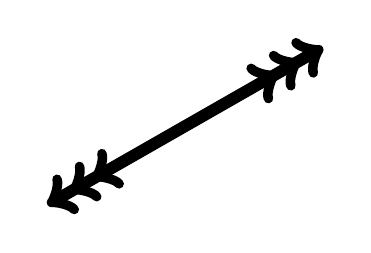
\begin{tikzpicture}
  \pgfsetarrows{<<<->>>}
  \pgfsetlinewidth{1ex}
  \pgfpathmoveto{\pgfpointorigin}
  \pgfpathlineto{\pgfpoint{3.5cm}{2cm}}
  \pgfusepath{stroke}
  \useasboundingbox (-0.25,-0.25) rectangle (3.75,2.25);
\end{tikzpicture}
\end{codeexample}
\end{command}





\subsection{Using an Arrow Tip Kind}

The following commands install the arrow kind that will be used when
stroking is done.

\begin{command}{\pgfsetarrowsstart\marg{start arrow kind}}
  Installs the given \meta{start arrow kind} for all subsequent
  strokes in the in the current \TeX-group. If \meta{start arrow kind}
  is empty, no arrow tips will be drawn at the start of the last
  segment of paths.
\begin{codeexample}[]
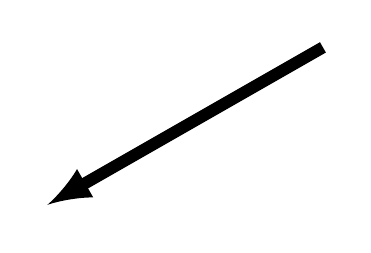
\begin{tikzpicture}
  \pgfsetarrowsstart{latex}
  \pgfsetlinewidth{1ex}
  \pgfpathmoveto{\pgfpointorigin}
  \pgfpathlineto{\pgfpoint{3.5cm}{2cm}}
  \pgfusepath{stroke}
  \useasboundingbox (-0.25,-0.25) rectangle (3.75,2.25);
\end{tikzpicture}
\end{codeexample}
\end{command}

\begin{command}{\pgfsetarrowsend\marg{start arrow kind}}
  Like |\pgfsetarrowsstart|, only for the end of the arrow.
\begin{codeexample}[]
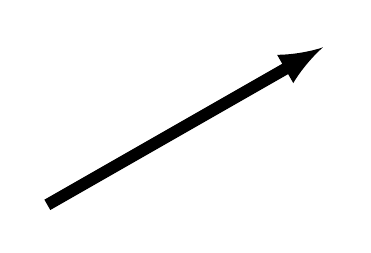
\begin{tikzpicture}
  \pgfsetarrowsend{latex}
  \pgfsetlinewidth{1ex}
  \pgfpathmoveto{\pgfpointorigin}
  \pgfpathlineto{\pgfpoint{3.5cm}{2cm}}
  \pgfusepath{stroke}
  \useasboundingbox (-0.25,-0.25) rectangle (3.75,2.25);
\end{tikzpicture}
\end{codeexample}
\end{command}

\emph{Warning:} If the compatibility mode is active (which is the
default), there also exist old commands called |\pgfsetstartarrow| and
|\pgfsetendarrow|, which are incompatible with the meta-arrow
management.


\begin{command}{\pgfsetarrows\texttt{\char`\{}\meta{start kind}|-|\meta{end kind}\texttt{\char`\}}}
  Calls |\pgfsetarrowsstart| for \meta{start kind} and
  |\pgfsetarrowsend| for \meta{end kind}.
\begin{codeexample}[]
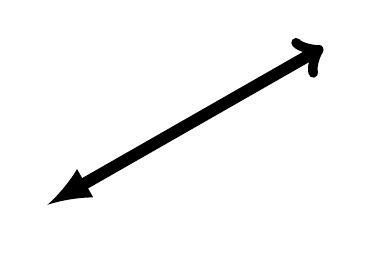
\begin{tikzpicture}
  \pgfsetarrows{latex-to}
  \pgfsetlinewidth{1ex}
  \pgfpathmoveto{\pgfpointorigin}
  \pgfpathlineto{\pgfpoint{3.5cm}{2cm}}
  \pgfusepath{stroke}
  \useasboundingbox (-0.25,-0.25) rectangle (3.75,2.25);
\end{tikzpicture}
\end{codeexample}
\end{command}


\subsection{Predefined Arrow Tip Kinds}

\label{standard-arrows}

The following arrow tip kinds are always defined:

{
\bigskip
\catcode`\|=12
\begin{tabular}{ll}
  \sarrow{stealth}{stealth} \\
  \sarrow{stealth reversed}{stealth reversed}  \\
  \sarrow{to}{to} \\
  \sarrow{to reversed}{to reversed}  \\
  \sarrow{latex}{latex} \\
  \sarrow{latex reversed}{latex reversed}  \\
  \index{*vbar@\protect\texttt{\protect\myvbar} arrow tip}%
  \index{Arrow tips!*vbar@\protect\texttt{\protect\myvbar}}
  \texttt{|-|}& yields thick
  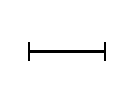
\begin{tikzpicture}[arrows={|-|},thick]
    \useasboundingbox (0pt,-0.5ex) rectangle (1cm,2ex);
    \draw (0,0) -- (1,0);
  \end{tikzpicture} and thin
  \begin{tikzpicture}[arrows={|-|},thin]
    \useasboundingbox (0pt,-0.5ex) rectangle (1cm,2ex);
    \draw (0,0) -- (1,0);
  \end{tikzpicture}
\end{tabular}
}

For further arrow tips, see page~\pageref{section-library-arrows}.

%%% Local Variables:
%%% mode: latex
%%% TeX-master: "pgfmanual"
%%% End:
